\chapter{Umsetzung und Ergebnisse}
\label{cha:umsetzung}

%Je nach Art der Arbeit kann diese Kapitelüberschrift auch \glqq Ergebnisse\grqq~lauten, z.~B. bei rein messtechnischen Aufgaben.

%Beschreibung der Umsetzung des zuvor gewählten Vorgehens (theoretische Untersuchung, Erhebungen, Durchführung von Experimenten, Prototypenaufbau, Implementierung eines Prozesses, etc.).

%Verifikation anhand der zuvor erarbeiteten Anforderungen und Validierung in Bezug auf das zuvor gestellte Ziel. Diskussion der Ergebnisse. Spätestens hier auch auf die Zuverlässigkeit der gewonnenen Erkenntnisse eingehen (z.~B. anhand der Genauigkeit von Messergebnissen).

Mechanischer Aufbau des LEGO-Spike-4-Gewinnt-Roboters


Für die Umsetzung des 4-Gewinnt-Roboters wurde eine mechanische Konstruktion gewählt, die es erlaubt, das Spielfeld zu scannen sowie Chips gezielt in eine Spalte einzuwerfen. Der Aufbau umfasst drei LEGO Spike-Motoren, einen Farbsensor und einen Drucktaster. Im Folgenden werden die einzelnen Komponenten detailliert beschrieben.

\begin{itemize}
	\item \textbf{Horizontalantrieb – Motor D}\\
	Der horizontale Antrieb des Farbsensors erfolgt über Motor D. Dieser ist dafür zuständig, die Spielfeldspalten nacheinander anzufahren. Der Motor ist mit einer Achse verbunden, welche zwei Räder antreiben. Die Bewegung erfolgt in gleichmäßigen Schritten: Eine Drehung um exakt 72 Grad bewegt den Schlitten um eine Spalte weiter. Diese Schrittweite wurde so gewählt, dass sie der Breite einer Spalte im Spielfeld entspricht. Dadurch ist eine exakte Positionierung des Sensors über jeder Spalte möglich, ohne dass zusätzliche Sensoren zur Positionsbestimmung notwendig sind. 
	\item \textbf{Vertikalantrieb – Motor E, Kette und Farbsensor}\\
	 Um das Spielfeld auch in vertikaler Richtung abfahren zu können, ist der Farbsensor an einer Kette montiert. Diese Kette wird durch Motor E angetrieben. Der Sensor ist an einem mittleren Segment der Kette befestigt und fährt beim Drehen der Kette entsprechend auf und ab. Ein Schritt des Motors um etwa 95 Grad bewegt den Sensor um genau eine Spielfeldhöhe weiter. Auf diese Weise können sämtliche sechs Reihen der aktuellen Spalte nacheinander abgescannt werden. Der Sensor wurde dabei so montiert, dass er exakt über der Mitte jedes Feldes positioniert ist, um eine zuverlässige Farberkennung zu ermöglichen. Die Rückwärtsbewegung der Kette erlaubt es, den Sensor wieder nach unten zu fahren.
	\item \textbf{Chipauswerfer – Motor A}\\
	Das Einwerfen des eigenen Spielsteins erfolgt über Motor A. An diesem Motor ist eine Stange montiert, die bei einer vollständigen Umdrehung einen Spielchip aus dem Vorratsmagazin in die gewünschte Spalte stößt. Nach der Auslösung kann ein neuer Chip in die Abschussposition nachrutschen. In der Software ist eine Wartezeit nach dem Auslösen eingebaut, damit der Chip sicher im Spielfeld ankommt, bevor die nächste Aktion beginnt.
	\item \textbf{Startsignal – Drucksensor (Force Sensor)}\\
	Um dem Roboter mitzuteilen, dass der menschliche Spieler seinen Zug abgeschlossen hat, wurde ein Drucksensor verwendet. Dieser befindet sich an der Vorderseite des Roboters. Sobald der Spieler den Sensor leicht berührt, wird ein Signal ausgelöst, das Prozess startet. 
	\item \textbf{Spielfeldscan – Farbsensor an Kette}\\
	 Für die Farberkennung des Spielfeldes wurde ein LEGO-Farbsensor verwendet, der über die oben beschriebene Kettenkonstruktion vertikal verfahrbar ist. Die Farbmessung erfolgt jeweils in der Mitte eines Spielfeldes. Der Sensor erkennt RGB-Werte, die per Software verschiedenen Spielsteinfarben (in diesem Projekt benutzt: Rot, Gelb oder Leer) zugeordnet werden. Während des Spiels vergleicht der Algorithmus die gemessenen Werte mit diesen Referenzwerten, um die tatsächliche Belegung jedes Feldes möglichst robust zu bestimmen. Der Abstand zwischen Sensor und Spielfeld beträgt etwa 7 mm – dieser Wert hat sich als optimal für zuverlässige Farbmessung erwiesen.
\end{itemize}
\textbf{Zusammenfassung}\\
Die mechanische Konstruktion basiert auf einem kartesischen Koordinatensystem, bei dem der Sensor durch die Kombination aus horizontaler (Motor D) und vertikaler Bewegung (Motor E + Kette) jede Spielfeldposition präzise anfahren kann. Das System erlaubt eine vollautomatische Spielweise: Der Roboter erkennt die aktuelle Spielsituation, berechnet den optimalen Zug und setzt diesen physisch um.


\begin{figure}[H]
	\centering
	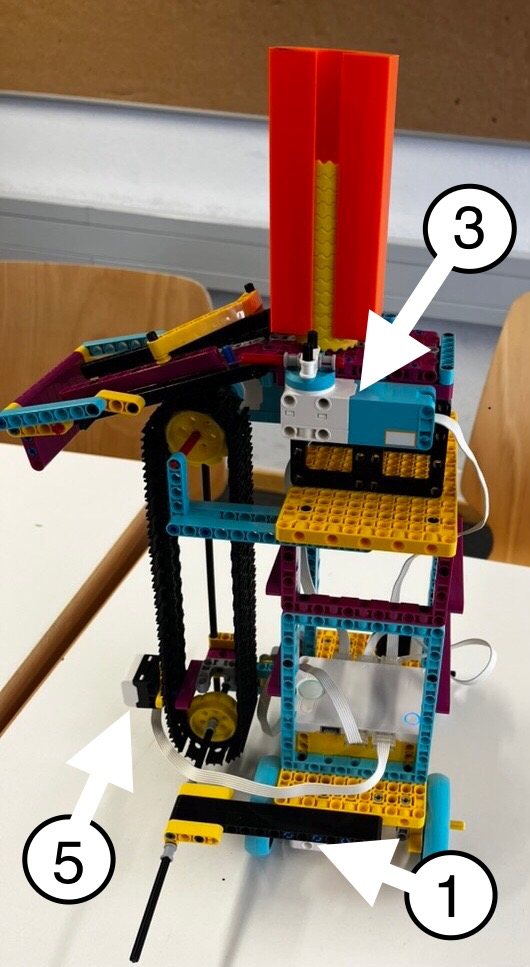
\includegraphics[width=0.5\linewidth]{images/188CF006-D571-4F2D-9337-8C4BDD7DAAEF_1_105_c}
	\caption{Seitenansicht links}
	\label{fig:188cf006-d571-4f2d-9337-8c4bdd7daaef1105c}
\end{figure}


\begin{figure}[H]
	\centering
	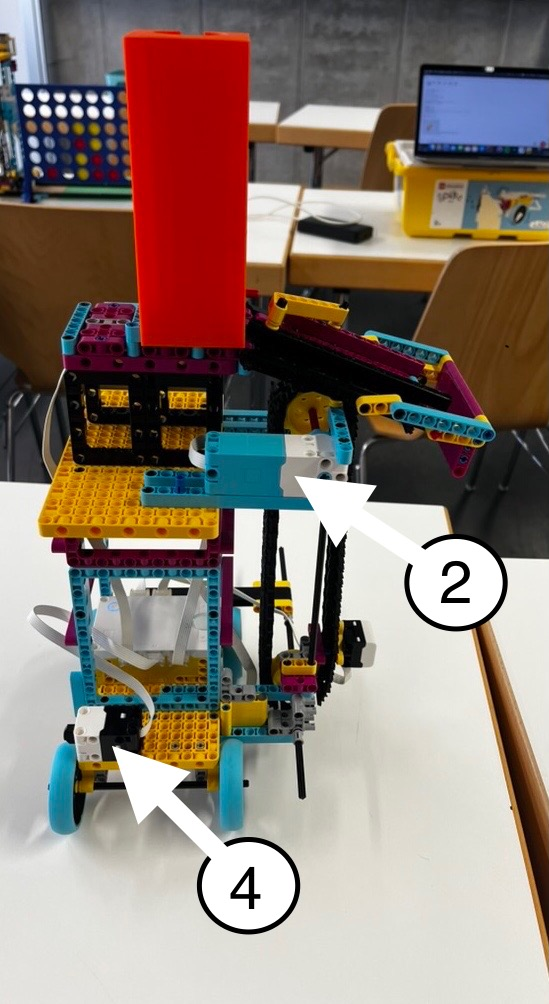
\includegraphics[width=0.5\linewidth]{images/DAE26A50-277E-4C6B-96A3-F2DE2CC9C004_1_105_c}
	\caption{Seitenansicht rechts}
	\label{fig:dae26a50-277e-4c6b-96a3-f2de2cc9c0041105c}
\end{figure}

